% ---
% Capitulo de revisão de literatura
% ---

\chapter{O Funcionamento dos Algoritmos}

\section{Insertion Sort}

O Insertion Sort é um algoritmo de classificação baseado em comparação local. Nele, um subconjunto do vetor é mantido como ordenado, o qual vai crescendo à medida que o vetor é percorrido e cada elemento é devidamente posicionado. Nesse posicionamento o novo item em foco tem que encontrar seu lugar apropriado e então ser inserido. Dessa característica origina o seu nome Insertion Sort, ou ordenação por inserção.

Em um passo-a-passo, o algoritmo segue as etapas abaixo ao percorrer o vetor:

\begin{itemize}

\item Se for o primeiro elemento, ele já está classificado.
\item Escolha o próximo elemento
\item Compare com todos os elementos na sub-lista classificada
\item Desloque todos os elementos na sub-lista classificada que são maiores que o valor a ser ordenado
\item Insira o valor
\item Repita até que a sub-lista classificada seja toda a lista

\end{itemize}

Um exemplo para ilustrar:

\begin{figure}[!htb]
\centering
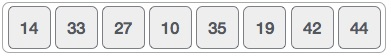
\includegraphics[width=9cm]{img/insertion_sort_1.jpg}
\caption{Parte-se de um vetor não ordenado}
\label{fig:insertion1}
\end{figure}

\begin{figure}[!htb]
\centering
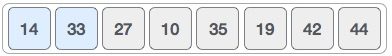
\includegraphics[width=9cm]{img/insertion_sort_2.jpg}
\caption{O Insertion Sort compara os dois primeiros elementos}
\label{fig:insertion2}
\end{figure}

\begin{figure}[!htb]
\centering
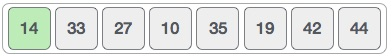
\includegraphics[width=9cm]{img/insertion_sort_3.jpg}
\caption{Os números 14 e 33 já estão ordenados de forma crescente. Neste momento, o elemento 14 é a sub-lista ordenada.}
\label{fig:insertion3}
\end{figure}

\begin{figure}[!htb]
\centering
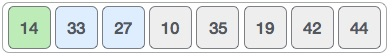
\includegraphics[width=9cm]{img/insertion_sort_4.jpg}
\caption{33 e 27 são comparados}
\label{fig:insertion4}
\end{figure}

\begin{figure}[!htb]
\centering
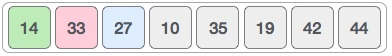
\includegraphics[width=9cm]{img/insertion_sort_5.jpg}
\caption{Neste caso, 33 está na posição incorreta}
\label{fig:insertion5}
\end{figure}

\begin{figure}[!htb]
\centering
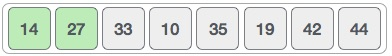
\includegraphics[width=9cm]{img/insertion_sort_6.jpg}
\caption{33 e 27 trocam de lugar. Ele também verifica todos os elementos da sub-lista ordenada. Aqui, vemos que a sub-lista classificada tem apenas um elemento 14, e 27 é maior que 14. Portanto, a sub-lista classificada permanece classificada após a troca. }
\label{fig:insertion6}
\end{figure}

\begin{figure}[!htb]
\centering
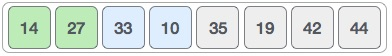
\includegraphics[width=9cm]{img/insertion_sort_7.jpg}
\caption{Agora 14 e 27 são a sub-lista ordenada. 33 e 10 são comparados}
\label{fig:insertion7}
\end{figure}

\begin{figure}[!htb]
\centering
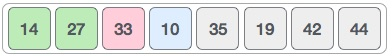
\includegraphics[width=9cm]{img/insertion_sort_8.jpg}
\caption{Eles não estão na ordem crescente correta}
\label{fig:insertion8}
\end{figure}

\begin{figure}[!htb]
\centering
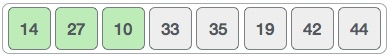
\includegraphics[width=9cm]{img/insertion_sort_9.jpg}
\caption{Trocam de lugar}
\label{fig:insertion9}
\end{figure}

\begin{figure}[!htb]
\centering
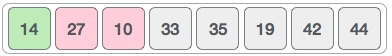
\includegraphics[width=9cm]{img/insertion_sort_10.jpg}
\caption{Entretanto, a sub-lista ainda não está ordenada corretamente, pois 10 ainda está após o 27}
\label{fig:insertion10}
\end{figure}

\begin{figure}[!htb]
\centering
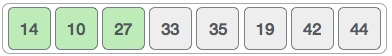
\includegraphics[width=9cm]{img/insertion_sort_11.jpg}
\caption{Então segue a troca}
\label{fig:insertion11}
\end{figure}

\begin{figure}[!htb]
\centering
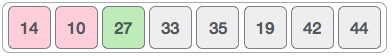
\includegraphics[width=9cm]{img/insertion_sort_12.jpg}
\caption{14 e 10 estão desordenados, então trocam de logar}
\label{fig:insertion12}
\end{figure}

\begin{figure}[!htb]
\centering
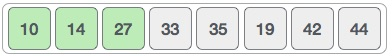
\includegraphics[width=9cm]{img/insertion_sort_13.jpg}
\caption{Ao fim da terceira iteração, temos uma sub-lista ordenada de 4 itens. O processo segue iterativamente.}
\label{fig:insertion13}
\end{figure}

\section{Merge Sort}

O Merge Sort é um dos algoritmos de classificação mais eficientes. Ele tem como princípio de funcionamento a divisão e conquista. O algoritmo divide repetidamente uma lista em várias sublistas até que cada sublista consista em um único elemento, e ao retornar mesclando essas sublistas ordenadamente, obtém-se a lista original de forma ordenada. Esse processo pode ser descrito pelos passos a seguir:

\begin{itemize}

	\item Se houver apenas 1 elemento na lista, está ordenado, retorne
	\item Divida a lista recursivamente ao meio até que não possa ser mais dividida
	\item Mescle as listas menores em uma nova lista ordenada

\end{itemize}

Para ilustrar o funcionamento, toma-se como exemplo de partida o vetor abaixo.

\begin{figure}[!htb]
\centering
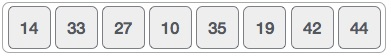
\includegraphics[width=9cm]{img/merge1.jpg}
\label{fig:merge1}
\end{figure}

Sabemos que o Merge Sort primeiro divide todo o vetor iterativamente em metades iguais, até que os elementos singulares sejam alcançados. Vemos aqui que um vetor de 8 itens é dividida em dois vetores de tamanho 4. 

\begin{figure}[!htb]
\centering
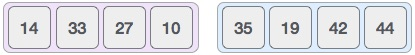
\includegraphics[width=9cm]{img/merge2.jpg}
\label{fig:merge2}
\end{figure}

Isso não altera a seqüência dos itens. Agora dividimos esses dois vetores em metades. 

\begin{figure}[!htb]
\centering
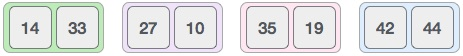
\includegraphics[width=9cm]{img/merge3.jpg}
\label{fig:merge3}
\end{figure}

Nós dividimos ainda mais esses vetores e alcançamos o valor único que não pode mais ser dividido. 

\begin{figure}[!htb]
\centering
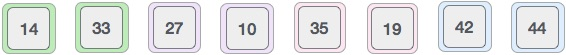
\includegraphics[width=9cm]{img/merge4.jpg}
\label{fig:merge4}
\end{figure}

Agora, nós os combinamos exatamente da mesma maneira como foram divididos. Observe as cores dadas a essas listas. Primeiro comparamos o elemento de cada lista e, em seguida, os combinamos em outra lista de maneira ordenada. Vemos que 14 e 33 estão em posições ordenadas. Comparamos 27 e 10 e na lista de destino de 2 valores colocamos 10 primeiro, seguido por 27. Alteramos a ordem de 19 e 35, enquanto 42 e 44 são colocados sequencialmente. 

\begin{figure}[!htb]
\centering
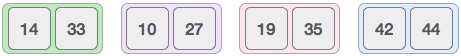
\includegraphics[width=9cm]{img/merge5.jpg}
\label{fig:merge5}
\end{figure}

Na próxima iteração da fase de mesclagem, dois índices iteram sobre os conjuntos, de forma que se compara o menor elemento corrente de um conjunto com o menor elemento corrente do outro. Dessa forma, ao retirar os elementos um a um, de forma ordenada, obtém-se uma nova sub-lista ordenada.

\begin{figure}[!htb]
\centering
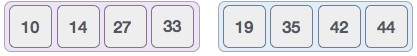
\includegraphics[width=9cm]{img/merge6.jpg}
\label{fig:merge6}
\end{figure}

Após a última mesclagem, a lista original encontra-se ordenada

\begin{figure}[!htb]
\centering
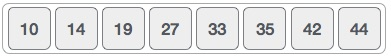
\includegraphics[width=9cm]{img/merge7.jpg}
\label{fig:merge7}
\end{figure}

\section{Tim Sort}

O Tim Sort foi implementado pela primeira vez em 2002 por Tim Peters para uso em Python. Supostamente, veio do entendimento de que a maioria dos algoritmos de classificação nascem em salas de aula e não são projetados para uso prático em dados do mundo real. Tim Sort tira proveito de padrões comuns em dados e utiliza uma combinação de Merge Sort e Insertion Sort junto com alguma lógica interna para otimizar a manipulação de dados em grande escala.

A chave para entender a implementação de Tim Sort é entender o conceito de \textit{runs}. O Tim Sort aproveita os dados pré-classificados que ocorrem naturalmente a seu favor. Por pré-ordenado, simplesmente queremos dizer que os elementos sequenciais estão todos aumentando ou diminuindo (não nos importamos com quais). Em um passo a passo, o algoritmo pode ser descrito da seguinte maneira:

\begin{itemize}

\item Estabeleça um tamanho de minrun que seja uma potência de 2 (geralmente 32, nunca mais que 64 ou seu Insertion Sort perderá eficiência)
\item Encontrar uma run, uma sub-lista que se estenda enquanto os elementos estiverem ordenados, mas que tenha, pelo menos a quantidade minrun de elementos.
\item Se a run não tiver a quantidade mínima do minrun, usar o Insertion Sort para pegar os itens subsequentes ou anteriores e inseri-los na run até que tenha o tamanho mínimo correto.
\item Repita até que todo o vetor seja dividido em subseções classificadas.
\item Usar o merge do Merge Sort para unir os vetores ordenados. 


\end{itemize}

\section{Análise de Complexidade}

A análise de complexidade do algoritmo é projetada para comparar dois algoritmos em um nível teórico - ignorando detalhes de baixo nível, como a linguagem de programação, o hardware em que o algoritmo é executado ou o conjunto de instruções de uma determinada CPU. O objetivo é comparar algoritmos em termos das operações relevantes que são executadas na rotina. Um algoritmo ruim escrito em uma linguagem de programação de baixo nível, como assembly, pode executar muito mais rápido do que um bom algoritmo escrito em uma linguagem de programação de alto nível, como Python ou Ruby. Portanto, a análise de complexidade provê um parâmetro do que realmente é um "algoritmo melhor". 

Essa análise é feita em 3 cenários: melhor caso, pior caso e caso médio. A ocorrência de um cenário particular depende do formato da entrada a ser processada. No caso do Insertion Sort, por exemplo, o pior caso se dá quando a entrada está em ordem decrescente. Esse cenário faz com que o algoritmo percorra, no \textit{loop} interno, todas as posições possíveis para fazer a inserção do elemento. Como esse laço de repetição está dentro de uma iteração que percorre os N elementos do vetor, é dito que nesse pior caso a complexidade é O(n\textsuperscript{2}). A tabela abaixo exibe a complexidade dos algoritmos analisados e de antemão provê uma referência do seu comportamento à medida que o tamanho da entrada crescer durante a execução.

\begin{figure}[!htb]
\centering
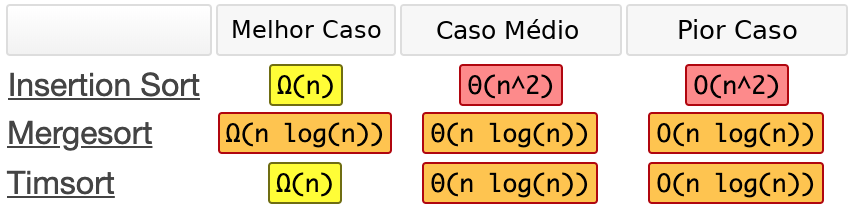
\includegraphics[width=10cm]{img/complexidade.png}
\caption{Análise de complexidade dos algoritmos em estudo}
\label{fig:complexidade}
\end{figure}
